%%%%%%%%%%%%%%%%%%%%%%%%%%%%%%%%%%%%%%%%%%%%%%%%%%%%%%%%%%%%%%%%%%%%%%%%
\section{Ausblick}
\begin{frame}
\frametitle{\kap. Ausblick}%
\tableofcontents[current]
\end{frame}
%%%%%%%%%%%%%%%%%%%%%%%%%%%%%%%%%%%%%%%%%%%%%%%%%%%%%%%%%%%%%%%%%%%%%%%%
\def\stitle{Guter Start ins Praktikum}%
\subsection{\stitle}\label{S:Guter Start}
\begin{frame}[t]%
  \frametitle{\kap.\ref{S:Guter Start} \stitle}%

In dieser \"Ubung wird anhand eines Beispiels beschrieben wie ein Java-Programm \"ubersichtlich gestaltet werden kann.

\begin{itemize}
    \item Wichtig f\"ur eigenes Verst\"andnis des Programms
    \item Wichtig f\"ur Dokumentation des Programms
    \item Wichtig f\"ur das Erhalten von Testaten
    \item Unwichtig f\"ur den Computer
\end{itemize}

\bigskip
\begin{block}{Programmierstil}
Einr\"ucken, Kommentare, Klammerung, Namen
\end{block}

\end{frame}

\def\stitle{Beispiel Obelisk}%
\subsection{\stitle}\label{S:Beispiel Obelisk}
\begin{frame}[t]%
    \frametitle{\kap.\ref{S:Beispiel Obelisk} \stitle}%

\begin{itemize}
 \item Ein \emph{Obelisk} ist ein Polyeder mit trapezf\"ormigen Seitenfl\"achen
 \item Es seien
 \begin{itemize}
  \item $a$ und $b$ die Seitenl\"angen der Grundfl\"ache
  \item $c$ und $d$ die Seitenl\"angen der Deckfl\"ache
  \item $h$ die H\"ohe des Obelisken
 \end{itemize}
\end{itemize}

\begin{center}
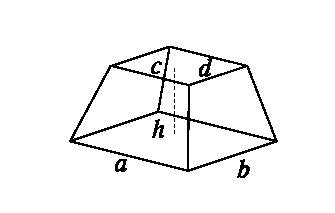
\includegraphics[width=0.5\textwidth]{\getexercisefolder bilder/obelisk}
\end{center}
\end{frame}


\def\stitle{Hilfsvariablen und Formeln}%
\subsection{\stitle}\label{S:Formeln}
\begin{frame}[t]%
    \frametitle{\kap.\ref{S:Formeln} \stitle}%

Dann ist:
\begin{itemize}
\item $G_1 = ab$ der Fl\"acheninhalt der Grundfl\"ache.
\item $G_2 = cd$ der Fl\"acheninhalt der Deckfl\"ache.
\item $\displaystyle A_1 = \frac{a+c}{2} \sqrt{h^2 + \Bigl(\frac{b-d}{2}\Bigr)^2}$
der Fl\"acheninhalt zweier Mantelfl\"achen.
\item $\displaystyle A_2 = \frac{b+d}{2} \sqrt{h^2 + \Bigl(\frac{a-c}{2}\Bigr)^2}$
der Fl\"acheninhalt der anderen beiden Mantelfl\"achen.
\item $M = 2 A_1 + 2 A_2$ der Fl\"acheninhalt der gesamten Mantelfl\"ache.
\item $O = M + G_1 + G_2$ der Fl\"acheninhalt der Oberfl\"ache .
\item $\displaystyle V = \frac{h}{6}\bigl(G_1 + (a+c)(b+d) + G_2\bigr)$ das Volumen.
\end{itemize}
\medskip

Schreiben Sie ein Java--Programm, welches die Seitenl\"angen $a$, $b$, $c$ und $d$ sowie die H\"ohe $h$ eines Obelisken von der Konsole einliest und anschlie\ss end den Fl\"acheninhalt der Mantelfl\"ache $M$, den der Oberfl\"ache $O$ sowie das Volumen $V$ ausgibt.

\end{frame}


\def\stitle{Programm: Schritt für Schritt}%
\subsection{\stitle}\label{S:Code}
\begin{frame}[fragile]%
    \frametitle{\kap.\ref{S:Code} \stitle}%
\heading{Programmgerüst}

\begin{lstlisting}[style=java]
/* Berechnung von
 * \ Mantelflaeche M
 * \ Oberflaeche O
 * \ Volumen V
 * eines Obelisken
 *
 * Eingabe: a,b,c,d (Seitenlaengen) h (Hoehe)
 * Ausgabe: M, O, V
 * Author: Stefan Findeisen 2016
 */
public class Obelisk {
  public static void main(String[] args)
  {
  /* Hier steht das Hauptprogramm */
  }
}
\end{lstlisting}
\end{frame}


\begin{frame}[fragile]%
    \frametitle{\kap.\ref{S:Code} \stitle}%
\heading{Lese Seitenlängen und Höhe ein}

\begin{lstlisting}[style=java]
public class Obelisk {
  public static void main(String[] args)
  {
    double a, b, c, d, h;
    Scanner sc = new Scanner(System.in);
    a = sc.nextDouble();
    b = sc.nextDouble();
    c = sc.nextDouble();
    d = sc.nextDouble();
    h = sc.nextDouble();
  }
}
\end{lstlisting}
\end{frame}


\begin{frame}[fragile]%
    \frametitle{\kap.\ref{S:Code} \stitle}%
\heading{Berechne Hilfsvariablen}

\begin{lstlisting}[style=java]
public class Obelisk {
  public static void main(String[] args)
  {
    /* Fortsetzung */
    double G1 = a * b;
    double G2 = c * d;
    double s1 = 0.5 * (a + c);
    double s2 = 0.5 * (b + d);
    double t1 = 0.5 * (b - d);
    double t2 = 0.5 * (a - c);
    double A1 = s1 * Math.sqrt(h * h + t1 * t1);
    double A2 = s2 * Math.sqrt(h * h + t2 * t2);
    double M = 2 * A1 + 2 * A2;
    double O = M + G1 + G2;
    double V = h / 6 * (G1 + (a + c) * (b + d) + G2);
  }
}
\end{lstlisting}
\end{frame}
